\section{Virtualios mašinos modelis}
	\subsection{Virtualios mašinos schema}
	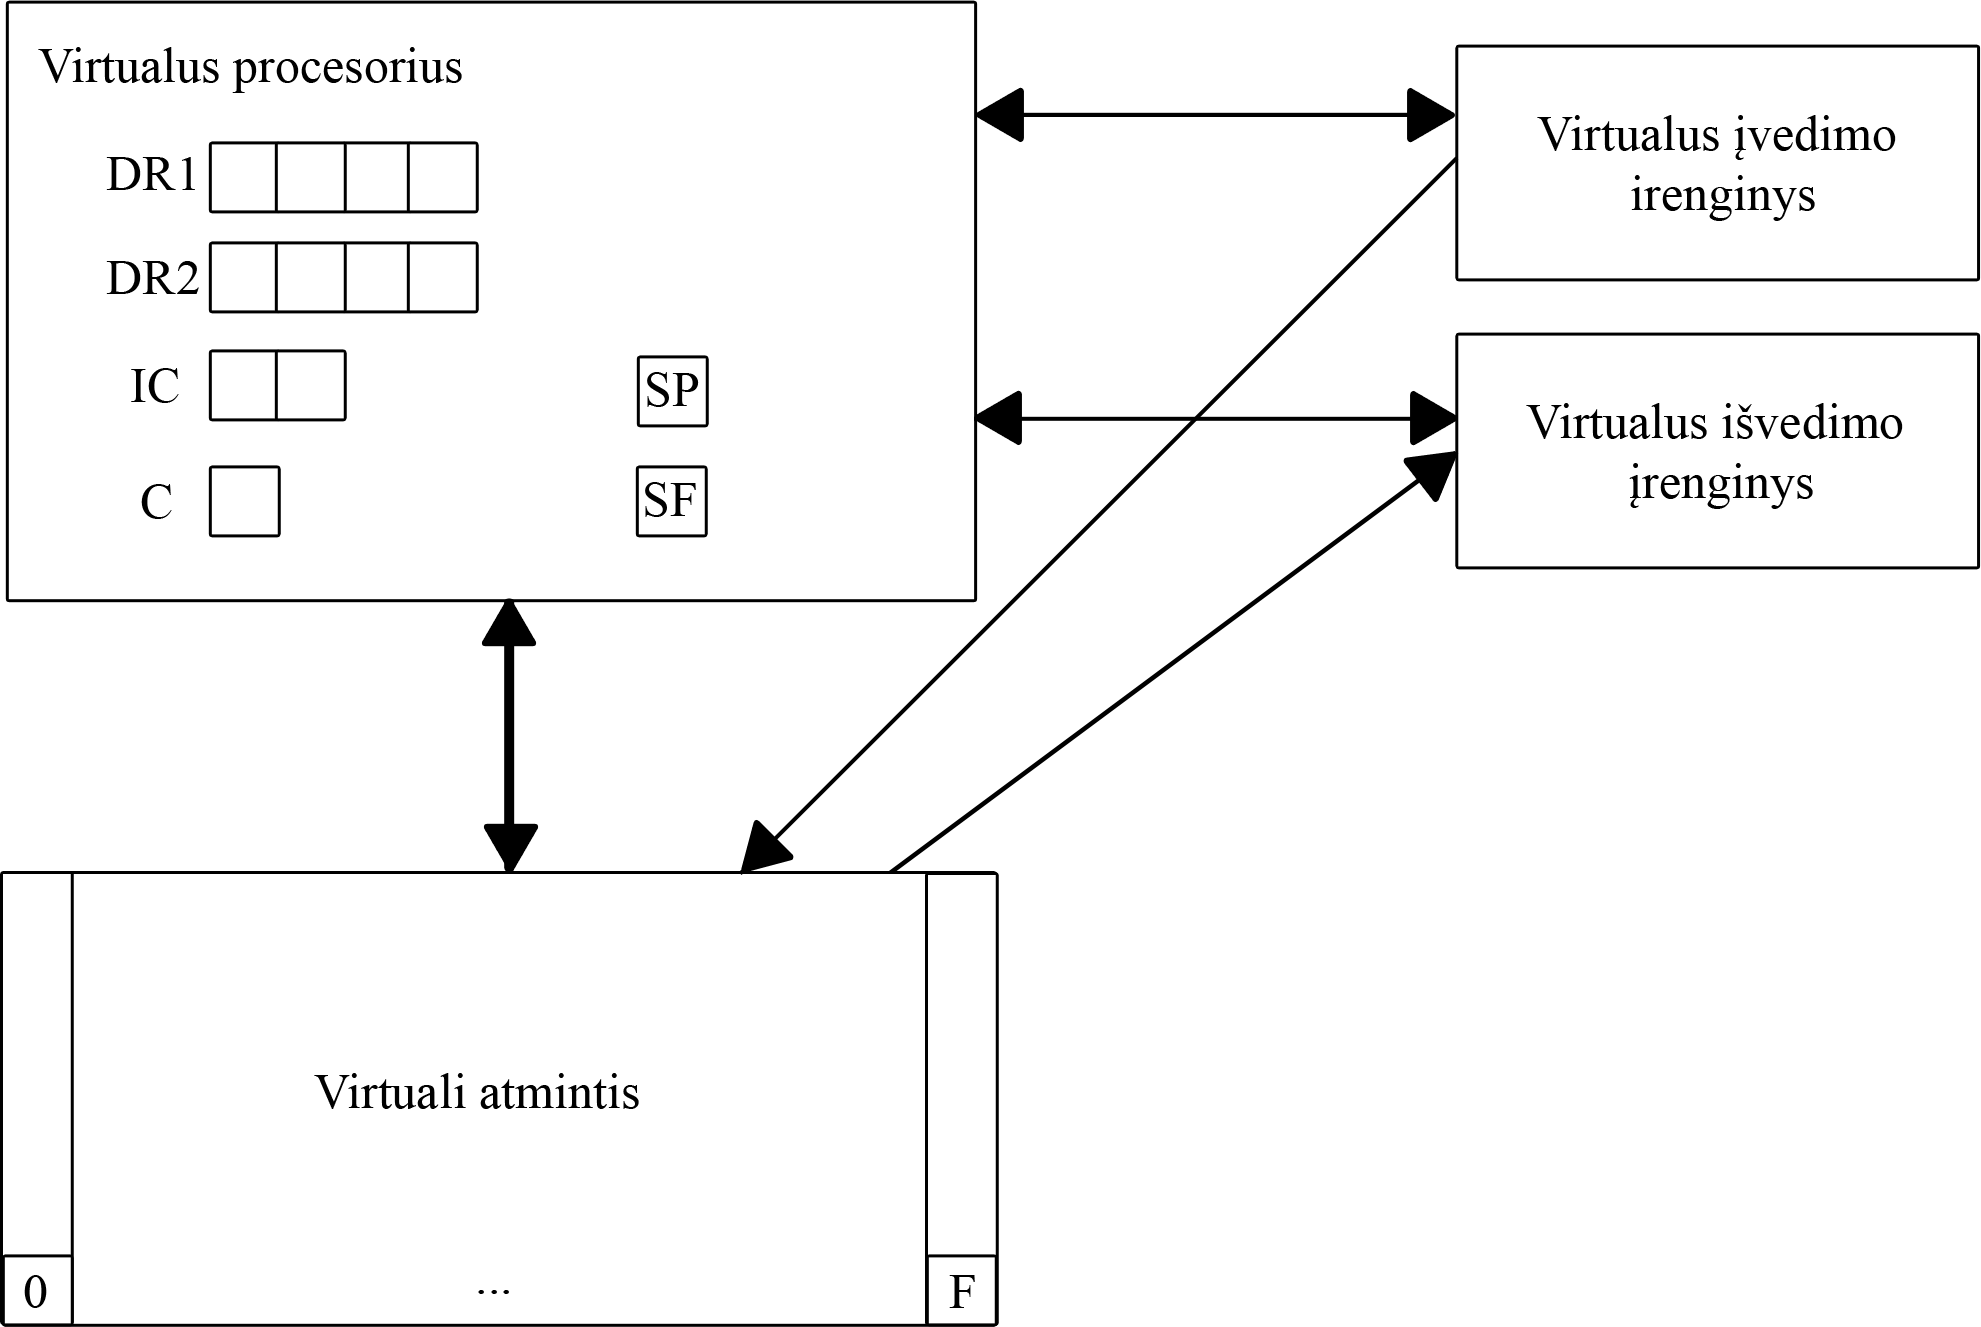
\includegraphics{VM.png}
	\subsection{Virtualios mašinos samprata}
	\textbf{Virtuali mašina} - tai tarsi realios mašinos kopija. Virtuali mašina yra sudaryta iš realios mašinos komponenčių, tokių kaip procesorius, atmintis, įvedimo/išvedimo įrenginiai. Jiems yra suteikiama paprastesnė nei reali vartotojo sąsaja.
	
	\subsection{Virtualios mašinos loginiai komponentai}
	\subsubsection{Virtualios mašinos atmintis}
	Virtualiai mašinai skirta 16 blokų po 16 žodžių, vieno žodžio dydis yra 32 bitai.
	
	Vienas blokas yra skirtas virtualios mašinos stekui.
	\subsubsection{Virtualios mašinos procesorius}
	Virtualios mašinos registrai:
	\begin{enumerate}
	\item Duomenų registrai: 
		\begin{itemize}
		\item DR1 - Data Register. Dydis - 4 baitai. Naudojamas duomenų pakrovimui į jį iš atminties ir iš jo į atmintį. Taip pat gali būti naudojamas operacijose.
		\item DR2 - Data Register. Dydis - 4 baitai. Naudojamas duomenų pakrovimui į jį iš atminties ir iš jo į atmintį. Taip pat gali būti naudojamas operacijose.
		\end{itemize}
	\item Segmentų registrai:
		\begin{itemize}
		\item CS - Code Segment. Rodyklė rodanti į kodo segmentą atmintyje.
		\item DS - Data Segment. Rodyklė rodanti į duomenų segmentą atmintyje.
		\item ST - Stack Segment. Rodyklė rodanti į steko segmentą atmintyje.
		\end{itemize}
	\item Nuorodų registrai:
		\begin{itemize}
		\item IC - Instruction Counter. Saugoma einamosios komandos žodžio indeksas.
		\item SP - Stack Pointer. Saugomas steko viršūnės žodžio indeksas.
		\end{itemize}
	\item Loginiai registrai:
		\begin{itemize}
		\item SF - Status Flag. Rodo procesoriaus būseną po aritmetinio veiksmo.
		\end{itemize}
	\end{enumerate}
	\subsubsection{Virtualios mašinos komandų sistema}
	Vieną komandą sudaro 4 baitai, tačiau nebūtinai visi baita privalo būti naudojami.
	\begin{enumerate}
	\item Aritmetinės komandos
		\begin{itemize}
		\item ADRR - sudeda registrus DR1 ir DR2. Rezultatas laikomas registre R1. Gali pakeisti visus flag'us.
		\item ADxy - sudeda registrą DR1 ir žodį esantį duomenų segmente adresu 10*x + y. Rezultatas laikomas registre DR1. Gali paskeisti visus flag'us.
		\item SBRR - atema DR2 reikšmę iš DR1. Rezultatas laikomas registre R1. Gali pakeisti visus flag'us.
		\item SBxy - atema žodį esantį duomenų segmente adresu 10*x + y iš registro DR1. Rezultatas laikomas registre DR1. Gali pakeisti visus flag'us.
		\item MLRR - sudaugina registrus DR1 ir DR2. Rezultatas laikomas registre DR1. Gali pakeisti visus flag'us.
		\item MLxy - sudaugina registrą DR1 iš žodžio esančio duomenų segmente adresu 10*x + y. Gali pakeisti visus flag'us.
		\item DVRR - padalina DR1 iš DR2. Dalybos rezultatas laikomas registre DR1, modulio rezultatas laikomas registre DR2. Gali pakeisti visus flag'us.
		\item DVxy - padalina DR1 iš žodžio esančio duomenų segmente adresu 10*x - y.
		\end{itemize}
	\item Loginės komandos
		\begin{itemize}
		\item AND - įvykdo AND operaciją tarp DR1 ir DR2. Rezultatas laikomas registre R1. Gali pakeisti ZF.
		\item OR - įvykdo OR operaciją tarp DR1 ir DR2. Rezultatas laikomas registre DR1. Gali pakeisti ZF.
		\item XOR - įvykdo XOR operaciją tarp DR1 ir DR2. Rezultatas laikomas registre DR1. Gali pakeisti ZF.
		\item NOT - įvykdo NOT operaciją DR1 registrui. Rezultatas laikomas registre DR1. Gali pakeisti ZF.
		\end{itemize}
	\item Palyginimo komandos
		\begin{itemize}
		\item CMP - palygina registrus DR1 ir DR2. Jei elementai lygūs, tada ZF = 1. Jei višutinis elementas didesnis, tada CF = 0 ir  ZF = 0. Jei viršutinis elementas mažesnis, CF = 1.
		\end{itemize}
	\item Darbo su duomenimis komandos
		\begin{itemize}
		\item LWxy - į DR1 įdedamas žodis esantis duomenų segmente adresu 10 * x + y.
		\item SWxy - į duomenų segmentą, adresu 10 * x + y įdedama DR1 reikšmė.
		\item MOV1 - į DR2 įdedama DR1 reikšmė.
		\item MOV2 - į DR1 įdedama DR2 reikšmė.
		\item PRNT - iškviečiamas pertraukimas, spausdinantis eilutę į ekraną. Eilutės adresas nurodytas registre DR1 viršūnėje, eilutės ilgis nurodytas registre DR2
		\item PRNS - iškviečiamas pertraukimas, DR1 reikšmę kaip skaičių į ekraną.
		\end{itemize}
	\item Darbo su steku komandos
		\begin{itemize}
		\item PUSH - steko viršūnės rodyklė padidinama vientu ir į steko viršūnę idedama DR1 reikšmė.
		\item POP - į DR1 įdedamas žodis esantis steko viršūnėje ir steko virūnės rodyklė sumažinama vienetu.
		\end{itemize}
	\item Valdymo perdavimo komandos
		\begin{itemize}
		\item JMxy - besąlyginio valdymo perdavimo komanda. Valdymas perduodamas kodo segmento žodžiui 10 * x + y, t.y. PC = 10 * x + y.
		\item JExy - sąlyginio valdymo perdavimo komanda. Jei ZF = 1 (elementai yra lygūs), tada valdymas perduodamas kodo segmento žodžiui 10 * x + y.
		\item JAxy - sąlyginio valdymo perdavimo komanda. Jei CF = 0 ir ZF = 0 (virūnės elementas yra didesnis), tada valdymas perduodamas kodo segmento žodžiui 10 * x + y.
		\item JLxy  - sąlyginio valdymo perdavimo komanda. Jei CF = 1 (viršūnės elementas yra mažesnis), tada valdymas perduodamas kodo segmento žodžiui 10 * x + y.
		\end{itemize}
	\item Failų rašymo, skaitymo komandos
		\begin{itemize}
		\item FOxy - Atidaromas failas esantis kietajame diske, failo pavadinimas yra xy. Failo handleris yra grąžinamas į DR1.
		\item FC - Uždaromas failas, DR1 yra šio failo handleris.
		\item FD - Ištrinamas failas, DR1 yra šio failo handleris.
		\item FRxy - DR1 yra failo handleris. 10*x + y nurodo vietą, į kurią rašysim duomenų segmente. DR2 nurodo adresą iš kurio skaitysim.
		\item FWxy - DR1 yra failo handleris. 10*x + y nurodo vietą, iš kurios rašysim iš duomenų segmento, DR2 nurodo adresą, kur įrašysim į failą.
		\end{itemize}
	\item Darbo pabaigos komanda
		\begin{itemize}
		\item HALT - parodo programos pabaigą.
		\end{itemize}
	\end{enumerate}
	Kodo struktūra turi būti tokia:\\
	DATASEG\\
	...\\
	CODESEG\\
	...\\
	HALT\\
	\\
	DATASEG viduje galima įdėti duomenis į duomenų segmentą naudojant DW komandą.
\clearpage